\begin{figure}[hbt!]
    \centering
    \begin{subfigure}[b]{0.6\textwidth}
        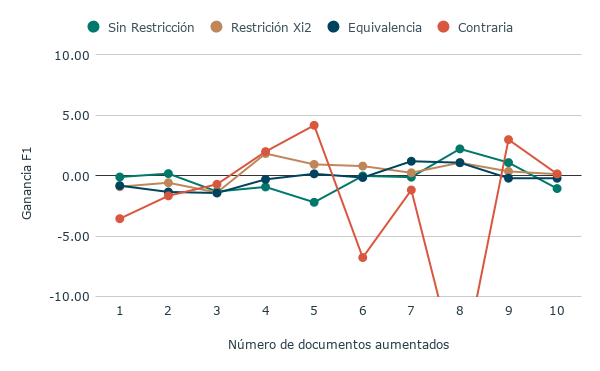
\includegraphics[width=\textwidth]{sections/figures/Bi-LSTM-anox.png}
        \caption{Bi-LSTM}
    \end{subfigure}
    \hfill
    
    \begin{subfigure}[b]{0.6\textwidth}
        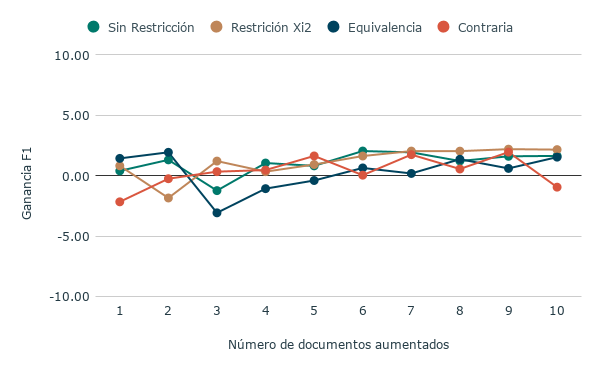
\includegraphics[width=\textwidth]{sections/figures/CNN_anox.png}
        \caption{CNN}
    \end{subfigure}

    
    \begin{subfigure}[b]{0.6\textwidth}
        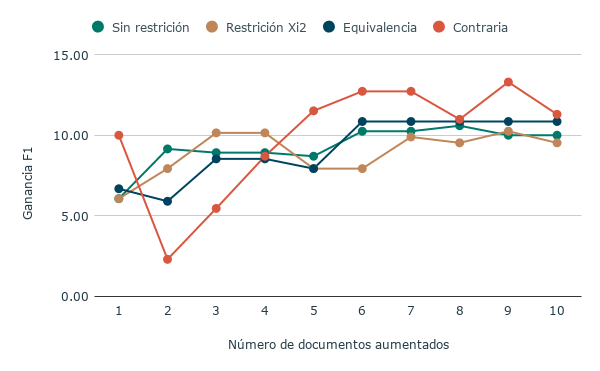
\includegraphics[width=\textwidth]{sections/figures/SVM-anorexia.png}
        \caption{SVM}
    \end{subfigure}
    
    \caption{Relación entre el número de documentos aumentados y la ganancia en F1 para el conjunto \textit{Anorexia}.}
    \label{fig:aumento_n_anorexia}
\end{figure}